\documentclass[10pt,a4paper]{article}
\usepackage[utf8]{inputenc}
\usepackage[T1]{fontenc}
\usepackage[spanish]{babel}
\usepackage{amsmath}
\usepackage{amsfonts}
\usepackage{amssymb}
\usepackage{graphicx}
\usepackage{subcaption}
\usepackage{lipsum}
\usepackage{multicol}
\usepackage[left=2.0cm, right=2.00cm, top=2.0cm, bottom=2.0cm]{geometry}

\author{Rondan Poma, Carlos Enrique}
\title{\LaTeX con Carlos}
\date{\today}



\begin{document}
	
	\maketitle
	\begin{center}
		\rule{15cm}{1pt}
		\begin{abstract}
			\lipsum[1] 
		\end{abstract}
		\rule{15cm}{1pt}
	\end{center}
	\tableofcontents
	\listoffigures
	\vspace{1cm}
	

	\begin{multicols}{2}
		\section{Introducción}
		\lipsum[2-6]
		\begin{figure*}
			\centering
			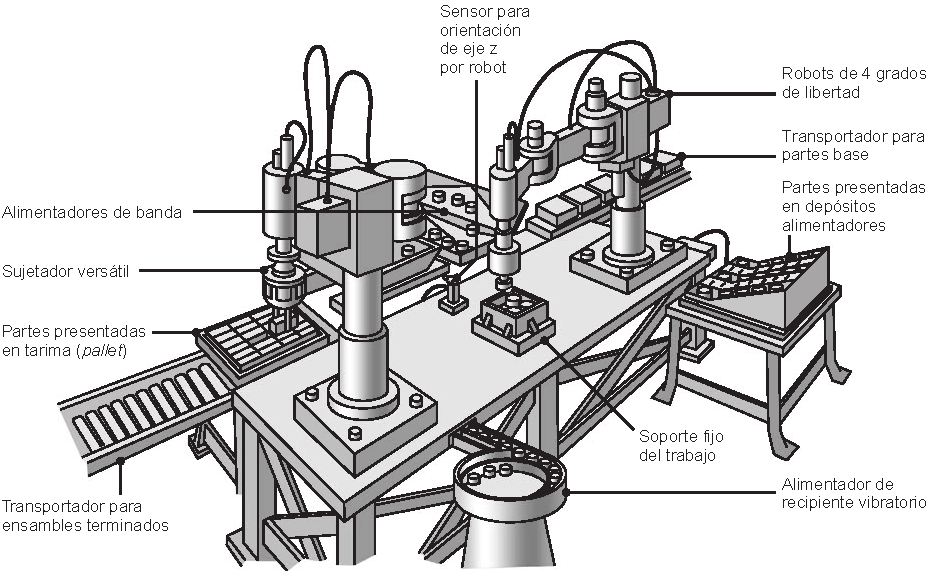
\includegraphics[width = \linewidth]{figuras/ensamble.pdf}
			\caption{Estación de ensamble de robot de dos brazos. Fuente: Product Design for Assembly, edición de 1989, de G. Boothroyd y P. Dewhurst. Reproducida con permiso}\label{fig:ensamble}
		\end{figure*}
		\section{Antecedentes}
		\lipsum[2-8]
		
		\section{Metodología}
		\subsection{CRISP-DM}
		\lipsum[2-6]
		\begin{figure*}
			\centering
			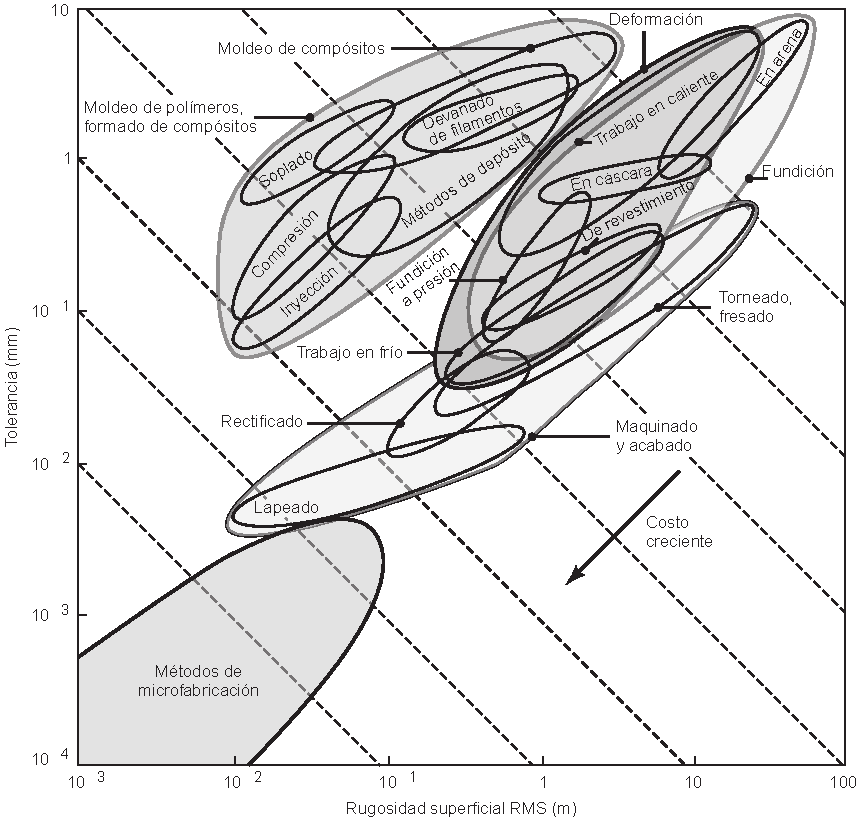
\includegraphics[width = 0.7\linewidth]{figuras/tolerancia}
			\caption{Gráfica de tolerancia obtenible contra rugosidad superficial para diversas operaciones de
				manufactura.}\label{fig:tolerancia}
		\end{figure*}
		\subsection{KDD}
		\lipsum[2-6] (ver figura \ref{fig:ensamble})
		%%%%%%%%%%%%%%%%%%%%%%%%%%%
		\begin{figure*}
			\centering
			\begin{subfigure}[b]{12cm}
				\centering
				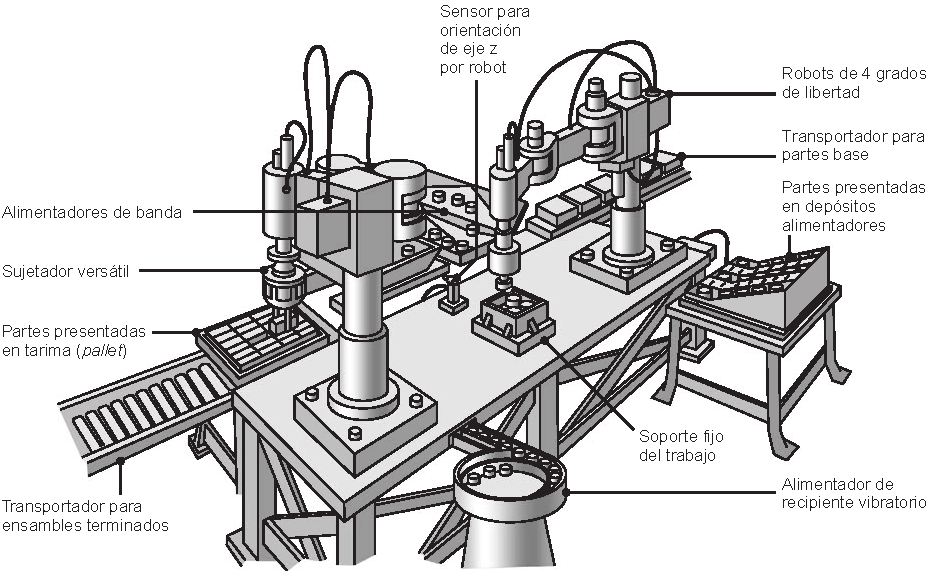
\includegraphics[width = 12cm]{figuras/ensamble.pdf}
				\caption{Estación de ensamble de robot de dos brazos. Fuente: Product Design for Assembly, edición de 1989, de G. Boothroyd y P. Dewhurst. Reproducida con permiso}
			\end{subfigure}\\
		\vspace{5mm}
			\begin{subfigure}[b]{12cm}
				\centering
				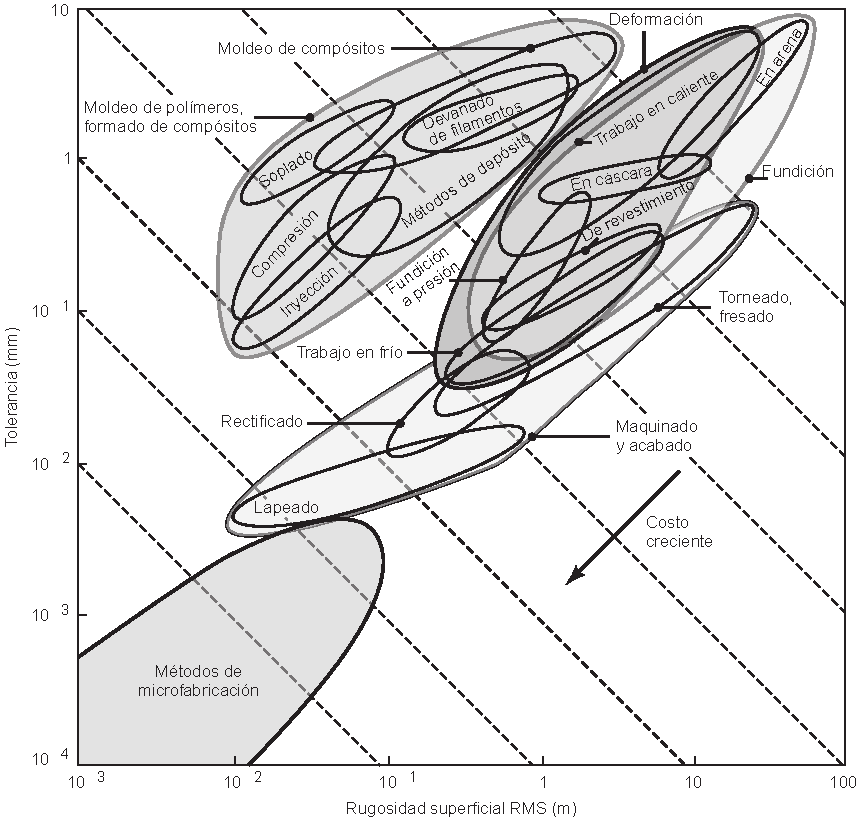
\includegraphics[width = 12cm]{figuras/tolerancia}
				\caption{Gráfica de tolerancia obtenible contra rugosidad superficial para diversas operaciones de manufactura.}
			\end{subfigure}
		\caption{Ejemplos de diseños indeseables (deficientes) y deseables (buenos) de fundición. }
		\end{figure*}
		%%%%%%%%%%%%%%%%%%%%%%%%%%%%%%%
		\section{Otros}
		\lipsum[2-6]
		(ver figura \ref{fig:tolerancia})
		
	\end{multicols}

	
\end{document}